Une comptabilité se fait entre des comptes bancaires, des comptes d'épargne
associés et des liquidités. Les comptes d'épargne dépendent entièrement d'un
compte courant (appelé bancaire ici) auquel ils sont associés. Les flux d'argent
se passent entre l'extérieur et un compte (utilisation de carte bleue), un compte
et une liquidité (retrait d'un compte), un compte et une épargne associée
(voir Fig.~\ref{compta:comptes}).
\begin{figure}
\centering
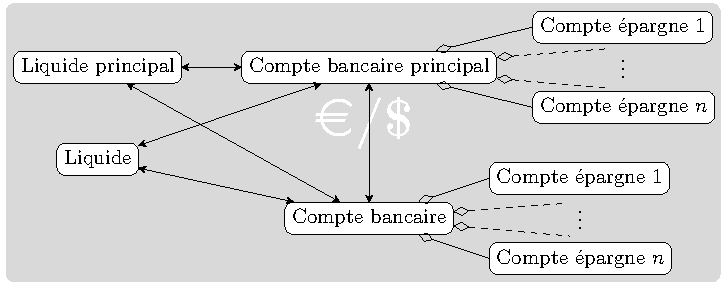
\includegraphics{entite}
\caption{\label{compta:comptes}Les comptes sont répartis entre comptes bancaires et
        comptes liquides. Tant qu'ils sont dans la même monnaie, ils peuvent tous
        interagir les uns avec les autres. Les comptes épargnes sont totalement gérés
        par le compte courant associé, rien ne peut en sortir/entrer sans passer
        par le compta bancaire.}
\end{figure}

Une tenue de comptabilité va consister à comptabiliser ces flux, les organiser
en catégories et comparer le total des flux avec des seuils. Il faut donc
un objet pour définir ces catégories et seuil: le prévisionnel.

\subsection{Prévisionnel}

Prévoir les dépenses peut se faire en les classant en catégories,
et en assignant à chacune d'elle un seuil à ne pas dépasser. 
La prédiction étant un art difficile,
et surtout lorsqu'il s'agit du futur\footnote{\og Prediction is very
difficult, especially about the futur.\fg\ \textsc{Niels Bohr}
(1885--1962)}, ce seuil peut se nuancer d'une certaine marge
pour le rendre flottant.
Ainsi chaque catégorie se caractérise par un nom, un seuil, mais
aussi une marge de man\oe uvre.

De plus, il est possible (et même fortement probable) qu'il existe des
opérations récurrentes tous les mois, typiquement des factures, 
un loyer, un prêt, etc. Ainsi il faut pouvoir ajouter
à certaines catégories des opérations qui, par hypothèse,
se passeront à un moment ou un autre dans le mois.

Un cran plus loin, il existe des opérations automatiques qui n'ont lieu qu'une
fois tous les deux mois, ou tous les $n$ mois de façon générale.
Il faut donc à chacune de ces opérations associer une période en
mois à laquelle il faut s'attendre à cette opération. Afin de bien
caractériser ce genre de comportement, il faut donc:
\begin{itemize}
\item une date de départ;
\item une date de fin;
\item une période;
\end{itemize}
pour une opération.

Au final, le prévisionnel est donc un ensemble de catégories, qui
peuvent contenir des sous-catégories afin de classer plus finement. Par
exemple on peut définir une catégorie \catForecast{Administratif}
qui regrouperait des transactions pour la nourriture, le transport,
etc. 

\`A cela, nous pouvons ajouter des opérations automatiques, par
exemple payer le loyer. Le loyer est payé tous les mois, il faut
donc s'y attendre s'il n'est pas passé. Un loyer ne dure que la période
pendant laquelle nous sommes locataires, autremement dit, une date de
début, une date de fin. De la même façon, la facture d'électricité doit
être payée, mais des fois tous les deux mois. Au final, notre catégorie
\catForecast{Administratif} peut se décrire ainsi:
\begin{itemize}
\item Transport, nourriture, etc;
\item \catForecast{Loyer}, de montant fixe, prévu tous les mois, pendant la période
                           de location;
\item \catForecast{Facture de gaz}, de montant prévu fixe, tous les deux mois,
                                    pendant la période dans un logement particulier.
\end{itemize}

\textit{In fine}, le prévisionnel est constitué de catégories, chacune pouvant
contenir des opérations attendues. Appelons \operation\ ces 
opérations attendues. Nous pouvons donc décrire le prévisionnel comme un 
ensemble de catégories contenant chacune un ensemble d'\operation s,
si par défaut une catégorie contient une \operation\ qui consiste
a attentre tout type de transaction dans ladîte catégorie, et possiblement
d'autres \operation s automatiques ou non, à attendre durant le mois.
La catégorie la plus petite est celle qui ne contient rien, ce qui
est équivalent à dire qu'elle ne contient qu'une \operation: l'\operation\
par défaut décrite plus haut.

Le but d'un prévisionnel est de pouvoir fournir chaque mois le montant total
et par catégorie, avec sa marge associée, à ne pas dépasser.

\subsection{Compte bancaire}
\subsubsection{Compte courant}
Un compte bancaire se compose d'un compte courant auquel
on associe une ou plusieurs épargnes. Un compte courant
a un historique et une monnaie.
\subsubsection{Compte épargne}
Un compte épargne a la monnaie de son compte courant associé, toutes
ses opérations sont liées au compte courant.
\subsection{Liquide}
Identique au compte bancaire, sans épargne.
